\documentclass[1p]{elsarticle_modified}
%\bibliographystyle{elsarticle-num}

%\usepackage[colorlinks]{hyperref}
%\usepackage{abbrmath_seonhwa} %\Abb, \Ascr, \Acal ,\Abf, \Afrak
\usepackage{amsfonts}
\usepackage{amssymb}
\usepackage{amsmath}
\usepackage{amsthm}
\usepackage{scalefnt}
\usepackage{amsbsy}
\usepackage{kotex}
\usepackage{caption}
\usepackage{subfig}
\usepackage{color}
\usepackage{graphicx}
\usepackage{xcolor} %% white, black, red, green, blue, cyan, magenta, yellow
\usepackage{float}
\usepackage{setspace}
\usepackage{hyperref}

\usepackage{tikz}
\usetikzlibrary{arrows}

\usepackage{multirow}
\usepackage{array} % fixed length table
\usepackage{hhline}

%%%%%%%%%%%%%%%%%%%%%
\makeatletter
\renewcommand*\env@matrix[1][\arraystretch]{%
	\edef\arraystretch{#1}%
	\hskip -\arraycolsep
	\let\@ifnextchar\new@ifnextchar
	\array{*\c@MaxMatrixCols c}}
\makeatother %https://tex.stackexchange.com/questions/14071/how-can-i-increase-the-line-spacing-in-a-matrix
%%%%%%%%%%%%%%%

\usepackage[normalem]{ulem}

\newcommand{\msout}[1]{\ifmmode\text{\sout{\ensuremath{#1}}}\else\sout{#1}\fi}
%SOURCE: \msout is \stkout macro in https://tex.stackexchange.com/questions/20609/strikeout-in-math-mode

\newcommand{\cancel}[1]{
	\ifmmode
	{\color{red}\msout{#1}}
	\else
	{\color{red}\sout{#1}}
	\fi
}

\newcommand{\add}[1]{
	{\color{blue}\uwave{#1}}
}

\newcommand{\replace}[2]{
	\ifmmode
	{\color{red}\msout{#1}}{\color{blue}\uwave{#2}}
	\else
	{\color{red}\sout{#1}}{\color{blue}\uwave{#2}}
	\fi
}

\newcommand{\Sol}{\mathcal{S}} %segment
\newcommand{\D}{D} %diagram
\newcommand{\A}{\mathcal{A}} %arc


%%%%%%%%%%%%%%%%%%%%%%%%%%%%%5 test

\def\sl{\operatorname{\textup{SL}}(2,\Cbb)}
\def\psl{\operatorname{\textup{PSL}}(2,\Cbb)}
\def\quan{\mkern 1mu \triangleright \mkern 1mu}

\theoremstyle{definition}
\newtheorem{thm}{Theorem}[section]
\newtheorem{prop}[thm]{Proposition}
\newtheorem{lem}[thm]{Lemma}
\newtheorem{ques}[thm]{Question}
\newtheorem{cor}[thm]{Corollary}
\newtheorem{defn}[thm]{Definition}
\newtheorem{exam}[thm]{Example}
\newtheorem{rmk}[thm]{Remark}
\newtheorem{alg}[thm]{Algorithm}

\newcommand{\I}{\sqrt{-1}}
\begin{document}

%\begin{frontmatter}
%
%\title{Boundary parabolic representations of knots up to 8 crossings}
%
%%% Group authors per affiliation:
%\author{Yunhi Cho} 
%\address{Department of Mathematics, University of Seoul, Seoul, Korea}
%\ead{yhcho@uos.ac.kr}
%
%
%\author{Seonhwa Kim} %\fnref{s_kim}}
%\address{Center for Geometry and Physics, Institute for Basic Science, Pohang, 37673, Korea}
%\ead{ryeona17@ibs.re.kr}
%
%\author{Hyuk Kim}
%\address{Department of Mathematical Sciences, Seoul National University, Seoul 08826, Korea}
%\ead{hyukkim@snu.ac.kr}
%
%\author{Seokbeom Yoon}
%\address{Department of Mathematical Sciences, Seoul National University, Seoul, 08826,  Korea}
%\ead{sbyoon15@snu.ac.kr}
%
%\begin{abstract}
%We find all boundary parabolic representation of knots up to 8 crossings.
%
%\end{abstract}
%\begin{keyword}
%    \MSC[2010] 57M25 
%\end{keyword}
%
%\end{frontmatter}

%\linenumbers
%\tableofcontents
%
\newcommand\colored[1]{\textcolor{white}{\rule[-0.35ex]{0.8em}{1.4ex}}\kern-0.8em\color{red} #1}%
%\newcommand\colored[1]{\textcolor{white}{ #1}\kern-2.17ex	\textcolor{white}{ #1}\kern-1.81ex	\textcolor{white}{ #1}\kern-2.15ex\color{red}#1	}

{\Large $\underline{12a_{0593}~(K12a_{0593})}$}

\setlength{\tabcolsep}{10pt}
\renewcommand{\arraystretch}{1.6}
\vspace{1cm}\begin{tabular}{m{100pt}>{\centering\arraybackslash}m{274pt}}
\multirow{5}{120pt}{
	\centering
	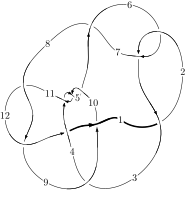
\includegraphics[width=112pt]{../../../GIT/diagram.site/Diagrams/png/1394_12a_0593.png}\\
\ \ \ A knot diagram\footnotemark}&
\allowdisplaybreaks
\textbf{Linearized knot diagam} \\
\cline{2-2}
 &
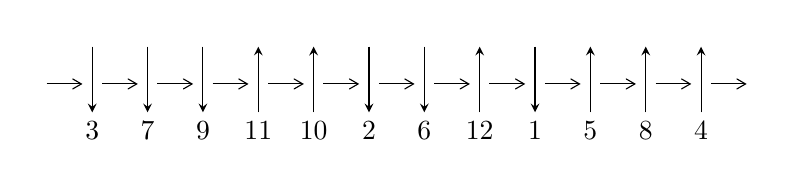
\begin{tikzpicture}[x=20pt, y=17pt]
	% nodes
	\node (C0) at (0, 0) {};
	\node (C1) at (1, 0) {};
	\node (C1U) at (1, +1) {};
	\node (C1D) at (1, -1) {3};

	\node (C2) at (2, 0) {};
	\node (C2U) at (2, +1) {};
	\node (C2D) at (2, -1) {7};

	\node (C3) at (3, 0) {};
	\node (C3U) at (3, +1) {};
	\node (C3D) at (3, -1) {9};

	\node (C4) at (4, 0) {};
	\node (C4U) at (4, +1) {};
	\node (C4D) at (4, -1) {11};

	\node (C5) at (5, 0) {};
	\node (C5U) at (5, +1) {};
	\node (C5D) at (5, -1) {10};

	\node (C6) at (6, 0) {};
	\node (C6U) at (6, +1) {};
	\node (C6D) at (6, -1) {2};

	\node (C7) at (7, 0) {};
	\node (C7U) at (7, +1) {};
	\node (C7D) at (7, -1) {6};

	\node (C8) at (8, 0) {};
	\node (C8U) at (8, +1) {};
	\node (C8D) at (8, -1) {12};

	\node (C9) at (9, 0) {};
	\node (C9U) at (9, +1) {};
	\node (C9D) at (9, -1) {1};

	\node (C10) at (10, 0) {};
	\node (C10U) at (10, +1) {};
	\node (C10D) at (10, -1) {5};

	\node (C11) at (11, 0) {};
	\node (C11U) at (11, +1) {};
	\node (C11D) at (11, -1) {8};

	\node (C12) at (12, 0) {};
	\node (C12U) at (12, +1) {};
	\node (C12D) at (12, -1) {4};
	\node (C13) at (13, 0) {};

	% arrows
	\draw[->,>={angle 60}]
	(C0) edge (C1) (C1) edge (C2) (C2) edge (C3) (C3) edge (C4) (C4) edge (C5) (C5) edge (C6) (C6) edge (C7) (C7) edge (C8) (C8) edge (C9) (C9) edge (C10) (C10) edge (C11) (C11) edge (C12) (C12) edge (C13) ;	\draw[->,>=stealth]
	(C1U) edge (C1D) (C2U) edge (C2D) (C3U) edge (C3D) (C4D) edge (C4U) (C5D) edge (C5U) (C6U) edge (C6D) (C7U) edge (C7D) (C8D) edge (C8U) (C9U) edge (C9D) (C10D) edge (C10U) (C11D) edge (C11U) (C12D) edge (C12U) ;
	\end{tikzpicture} \\
\hhline{~~} \\& 
\textbf{Solving Sequence} \\ \cline{2-2} 
 &
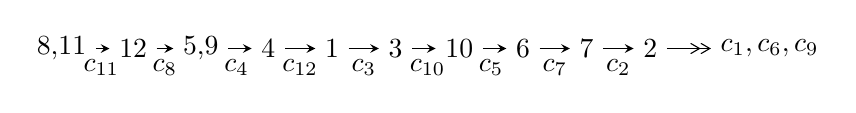
\begin{tikzpicture}[x=23pt, y=7pt]
	% node
	\node (A0) at (-1/8, 0) {8,11};
	\node (A1) at (1, 0) {12};
	\node (A2) at (33/16, 0) {5,9};
	\node (A3) at (25/8, 0) {4};
	\node (A4) at (33/8, 0) {1};
	\node (A5) at (41/8, 0) {3};
	\node (A6) at (49/8, 0) {10};
	\node (A7) at (57/8, 0) {6};
	\node (A8) at (65/8, 0) {7};
	\node (A9) at (73/8, 0) {2};
	\node (C1) at (1/2, -1) {$c_{11}$};
	\node (C2) at (3/2, -1) {$c_{8}$};
	\node (C3) at (21/8, -1) {$c_{4}$};
	\node (C4) at (29/8, -1) {$c_{12}$};
	\node (C5) at (37/8, -1) {$c_{3}$};
	\node (C6) at (45/8, -1) {$c_{10}$};
	\node (C7) at (53/8, -1) {$c_{5}$};
	\node (C8) at (61/8, -1) {$c_{7}$};
	\node (C9) at (69/8, -1) {$c_{2}$};
	\node (A10) at (11, 0) {$c_{1},c_{6},c_{9}$};

	% edge
	\draw[->,>=stealth]	
	(A0) edge (A1) (A1) edge (A2) (A2) edge (A3) (A3) edge (A4) (A4) edge (A5) (A5) edge (A6) (A6) edge (A7) (A7) edge (A8) (A8) edge (A9) ;
	\draw[->>,>={angle 60}]	
	(A9) edge (A10);
\end{tikzpicture} \\ 

\end{tabular} \\

\footnotetext{
The image of knot diagram is generated by the software ``\textbf{Draw programme}" developed by Andrew Bartholomew(\url{http://www.layer8.co.uk/maths/draw/index.htm\#Running-draw}), where we modified some parts for our purpose(\url{https://github.com/CATsTAILs/LinksPainter}).
}\phantom \\ \newline 
\centering \textbf{Ideals for irreducible components\footnotemark of $X_{\text{par}}$} 
 
\begin{align*}
I^u_{1}&=\langle 
-1.32744\times10^{451} u^{113}-2.40710\times10^{451} u^{112}+\cdots+1.44841\times10^{450} b+2.58438\times10^{453},\\
\phantom{I^u_{1}}&\phantom{= \langle  }-8.96722\times10^{451} u^{113}-1.11752\times10^{452} u^{112}+\cdots+1.88293\times10^{451} a+4.97987\times10^{454},\\
\phantom{I^u_{1}}&\phantom{= \langle  }u^{114}+u^{113}+\cdots-4199 u+169\rangle \\
I^u_{2}&=\langle 
-662 u^{23}-2292 u^{22}+\cdots+b-1244,\;-62 u^{23}-199 u^{22}+\cdots+a-70,\;u^{24}+4 u^{23}+\cdots+4 u+1\rangle \\
\\
\end{align*}
\raggedright * 2 irreducible components of $\dim_{\mathbb{C}}=0$, with total 138 representations.\\
\footnotetext{All coefficients of polynomials are rational numbers. But the coefficients are sometimes approximated in decimal forms when there is not enough margin.}
\newpage
\renewcommand{\arraystretch}{1}
\centering \section*{I. $I^u_{1}= \langle -1.33\times10^{451} u^{113}-2.41\times10^{451} u^{112}+\cdots+1.45\times10^{450} b+2.58\times10^{453},\;-8.97\times10^{451} u^{113}-1.12\times10^{452} u^{112}+\cdots+1.88\times10^{451} a+4.98\times10^{454},\;u^{114}+u^{113}+\cdots-4199 u+169 \rangle$}
\flushleft \textbf{(i) Arc colorings}\\
\begin{tabular}{m{7pt} m{180pt} m{7pt} m{180pt} }
\flushright $a_{8}=$&$\begin{pmatrix}0\\u\end{pmatrix}$ \\
\flushright $a_{11}=$&$\begin{pmatrix}1\\0\end{pmatrix}$ \\
\flushright $a_{12}=$&$\begin{pmatrix}1\\- u^2\end{pmatrix}$ \\
\flushright $a_{5}=$&$\begin{pmatrix}4.76238 u^{113}+5.93498 u^{112}+\cdots+57206.1 u-2644.75\\9.16483 u^{113}+16.6189 u^{112}+\cdots+42628.9 u-1784.29\end{pmatrix}$ \\
\flushright $a_{9}=$&$\begin{pmatrix}u\\- u^3+u\end{pmatrix}$ \\
\flushright $a_{4}=$&$\begin{pmatrix}-4.40245 u^{113}-10.6840 u^{112}+\cdots+14577.2 u-860.456\\9.16483 u^{113}+16.6189 u^{112}+\cdots+42628.9 u-1784.29\end{pmatrix}$ \\
\flushright $a_{1}=$&$\begin{pmatrix}-8.31120 u^{113}-14.8388 u^{112}+\cdots-44660.2 u+1930.35\\4.22266 u^{113}+6.63640 u^{112}+\cdots+26248.2 u-1124.56\end{pmatrix}$ \\
\flushright $a_{3}=$&$\begin{pmatrix}2.46989 u^{113}+1.67905 u^{112}+\cdots+47121.3 u-2220.56\\11.7433 u^{113}+21.3506 u^{112}+\cdots+53279.2 u-2216.47\end{pmatrix}$ \\
\flushright $a_{10}=$&$\begin{pmatrix}-8.93561 u^{113}-15.4866 u^{112}+\cdots-39386.1 u+1582.13\\-1.09804 u^{113}-2.20449 u^{112}+\cdots-4711.19 u+204.432\end{pmatrix}$ \\
\flushright $a_{6}=$&$\begin{pmatrix}11.2147 u^{113}+17.7407 u^{112}+\cdots+97403.9 u-4477.03\\-2.88475 u^{113}-5.30120 u^{112}+\cdots-18279.9 u+817.749\end{pmatrix}$ \\
\flushright $a_{7}=$&$\begin{pmatrix}1.86876 u^{113}+5.06983 u^{112}+\cdots-27684.6 u+1575.82\\1.21836 u^{113}+2.44360 u^{112}+\cdots+9086.94 u-438.831\end{pmatrix}$ \\
\flushright $a_{2}=$&$\begin{pmatrix}5.04895 u^{113}+7.19485 u^{112}+\cdots+56490.8 u-2694.95\\2.89155 u^{113}+5.23139 u^{112}+\cdots+10317.1 u-384.702\end{pmatrix}$\\&\end{tabular}
\flushleft \textbf{(ii) Obstruction class $= -1$}\\~\\
\flushleft \textbf{(iii) Cusp Shapes $= -6.63942 u^{113}-10.4925 u^{112}+\cdots-42753.9 u+1828.66$}\\~\\
\newpage\renewcommand{\arraystretch}{1}
\flushleft \textbf{(iv) u-Polynomials at the component}\newline \\
\begin{tabular}{m{50pt}|m{274pt}}
Crossings & \hspace{64pt}u-Polynomials at each crossing \\
\hline $$\begin{aligned}c_{1},c_{7}\end{aligned}$$&$\begin{aligned}
&u^{114}+37 u^{113}+\cdots+8270 u+361
\end{aligned}$\\
\hline $$\begin{aligned}c_{2},c_{6}\end{aligned}$$&$\begin{aligned}
&u^{114}- u^{113}+\cdots+66 u+19
\end{aligned}$\\
\hline $$\begin{aligned}c_{3}\end{aligned}$$&$\begin{aligned}
&u^{114}- u^{113}+\cdots-27558 u+8597
\end{aligned}$\\
\hline $$\begin{aligned}c_{4},c_{5},c_{10}\end{aligned}$$&$\begin{aligned}
&u^{114}- u^{113}+\cdots+769 u+229
\end{aligned}$\\
\hline $$\begin{aligned}c_{8},c_{11}\end{aligned}$$&$\begin{aligned}
&u^{114}+u^{113}+\cdots-4199 u+169
\end{aligned}$\\
\hline $$\begin{aligned}c_{9}\end{aligned}$$&$\begin{aligned}
&u^{114}+7 u^{113}+\cdots-5751 u+773
\end{aligned}$\\
\hline $$\begin{aligned}c_{12}\end{aligned}$$&$\begin{aligned}
&u^{114}+10 u^{113}+\cdots+31 u+1
\end{aligned}$\\
\hline
\end{tabular}\\~\\
\newpage\renewcommand{\arraystretch}{1}
\flushleft \textbf{(v) Riley Polynomials at the component}\newline \\
\begin{tabular}{m{50pt}|m{274pt}}
Crossings & \hspace{64pt}Riley Polynomials at each crossing \\
\hline $$\begin{aligned}c_{1},c_{7}\end{aligned}$$&$\begin{aligned}
&y^{114}+91 y^{113}+\cdots-5195518 y+130321
\end{aligned}$\\
\hline $$\begin{aligned}c_{2},c_{6}\end{aligned}$$&$\begin{aligned}
&y^{114}-37 y^{113}+\cdots-8270 y+361
\end{aligned}$\\
\hline $$\begin{aligned}c_{3}\end{aligned}$$&$\begin{aligned}
&y^{114}+41 y^{113}+\cdots+1509941114 y+73908409
\end{aligned}$\\
\hline $$\begin{aligned}c_{4},c_{5},c_{10}\end{aligned}$$&$\begin{aligned}
&y^{114}+109 y^{113}+\cdots-2438475 y+52441
\end{aligned}$\\
\hline $$\begin{aligned}c_{8},c_{11}\end{aligned}$$&$\begin{aligned}
&y^{114}-77 y^{113}+\cdots-3410251 y+28561
\end{aligned}$\\
\hline $$\begin{aligned}c_{9}\end{aligned}$$&$\begin{aligned}
&y^{114}+11 y^{113}+\cdots+25933727 y+597529
\end{aligned}$\\
\hline $$\begin{aligned}c_{12}\end{aligned}$$&$\begin{aligned}
&y^{114}-6 y^{113}+\cdots-317 y+1
\end{aligned}$\\
\hline
\end{tabular}\\~\\
\newpage\flushleft \textbf{(vi) Complex Volumes and Cusp Shapes}
$$\begin{array}{c|c|c}  
\text{Solutions to }I^u_{1}& \I (\text{vol} + \sqrt{-1}CS) & \text{Cusp shape}\\
 \hline 
\begin{aligned}
u &= -0.615929 + 0.781253 I \\
a &= \phantom{-}0.497409 + 1.316430 I \\
b &= \phantom{-}0.229336 + 1.327200 I\end{aligned}
 & -2.19312 - 0.80286 I & \phantom{-0.000000 } 0 \\ \hline\begin{aligned}
u &= -0.615929 - 0.781253 I \\
a &= \phantom{-}0.497409 - 1.316430 I \\
b &= \phantom{-}0.229336 - 1.327200 I\end{aligned}
 & -2.19312 + 0.80286 I & \phantom{-0.000000 } 0 \\ \hline\begin{aligned}
u &= -0.667133 + 0.720221 I \\
a &= -0.55170 - 1.32547 I \\
b &= -0.29464 - 1.41181 I\end{aligned}
 & -2.80844 + 4.84374 I & \phantom{-0.000000 } 0 \\ \hline\begin{aligned}
u &= -0.667133 - 0.720221 I \\
a &= -0.55170 + 1.32547 I \\
b &= -0.29464 + 1.41181 I\end{aligned}
 & -2.80844 - 4.84374 I & \phantom{-0.000000 } 0 \\ \hline\begin{aligned}
u &= -0.083165 + 0.969298 I \\
a &= \phantom{-}0.30191 + 1.77802 I \\
b &= -0.05886 + 1.42621 I\end{aligned}
 & -5.73613 - 2.30783 I & \phantom{-0.000000 } 0 \\ \hline\begin{aligned}
u &= -0.083165 - 0.969298 I \\
a &= \phantom{-}0.30191 - 1.77802 I \\
b &= -0.05886 - 1.42621 I\end{aligned}
 & -5.73613 + 2.30783 I & \phantom{-0.000000 } 0 \\ \hline\begin{aligned}
u &= \phantom{-}0.199303 + 1.011620 I \\
a &= -0.482565 + 0.090171 I \\
b &= -0.541287 - 0.234423 I\end{aligned}
 & \phantom{-}3.38338 + 1.88635 I & \phantom{-0.000000 } 0 \\ \hline\begin{aligned}
u &= \phantom{-}0.199303 - 1.011620 I \\
a &= -0.482565 - 0.090171 I \\
b &= -0.541287 + 0.234423 I\end{aligned}
 & \phantom{-}3.38338 - 1.88635 I & \phantom{-0.000000 } 0 \\ \hline\begin{aligned}
u &= \phantom{-}1.029690 + 0.157338 I \\
a &= -1.40100 + 1.63477 I \\
b &= \phantom{-}0.27627 + 1.39598 I\end{aligned}
 & \phantom{-}2.65526 + 2.33990 I & \phantom{-0.000000 } 0 \\ \hline\begin{aligned}
u &= \phantom{-}1.029690 - 0.157338 I \\
a &= -1.40100 - 1.63477 I \\
b &= \phantom{-}0.27627 - 1.39598 I\end{aligned}
 & \phantom{-}2.65526 - 2.33990 I & \phantom{-0.000000 } 0\\
 \hline 
 \end{array}$$\newpage$$\begin{array}{c|c|c}  
\text{Solutions to }I^u_{1}& \I (\text{vol} + \sqrt{-1}CS) & \text{Cusp shape}\\
 \hline 
\begin{aligned}
u &= \phantom{-}1.024990 + 0.209320 I \\
a &= \phantom{-}1.35036 - 1.94885 I \\
b &= -0.25017 - 1.46124 I\end{aligned}
 & \phantom{-}1.25171 + 8.39723 I & \phantom{-0.000000 } 0 \\ \hline\begin{aligned}
u &= \phantom{-}1.024990 - 0.209320 I \\
a &= \phantom{-}1.35036 + 1.94885 I \\
b &= -0.25017 + 1.46124 I\end{aligned}
 & \phantom{-}1.25171 - 8.39723 I & \phantom{-0.000000 } 0 \\ \hline\begin{aligned}
u &= \phantom{-}0.928859 + 0.161698 I \\
a &= \phantom{-}2.40502 - 1.28354 I \\
b &= -0.108151 - 1.331770 I\end{aligned}
 & -4.21976 + 0.72634 I & \phantom{-0.000000 } 0 \\ \hline\begin{aligned}
u &= \phantom{-}0.928859 - 0.161698 I \\
a &= \phantom{-}2.40502 + 1.28354 I \\
b &= -0.108151 + 1.331770 I\end{aligned}
 & -4.21976 - 0.72634 I & \phantom{-0.000000 } 0 \\ \hline\begin{aligned}
u &= \phantom{-}0.104528 + 1.054820 I \\
a &= \phantom{-}0.545595 + 0.008895 I \\
b &= \phantom{-}0.609233 + 0.283850 I\end{aligned}
 & \phantom{-}2.81497 + 7.66737 I & \phantom{-0.000000 } 0 \\ \hline\begin{aligned}
u &= \phantom{-}0.104528 - 1.054820 I \\
a &= \phantom{-}0.545595 - 0.008895 I \\
b &= \phantom{-}0.609233 - 0.283850 I\end{aligned}
 & \phantom{-}2.81497 - 7.66737 I & \phantom{-0.000000 } 0 \\ \hline\begin{aligned}
u &= -1.046020 + 0.191255 I \\
a &= \phantom{-}1.44286 - 0.22886 I \\
b &= -0.363035 + 0.092587 I\end{aligned}
 & -0.151342 - 0.849057 I & \phantom{-0.000000 } 0 \\ \hline\begin{aligned}
u &= -1.046020 - 0.191255 I \\
a &= \phantom{-}1.44286 + 0.22886 I \\
b &= -0.363035 - 0.092587 I\end{aligned}
 & -0.151342 + 0.849057 I & \phantom{-0.000000 } 0 \\ \hline\begin{aligned}
u &= -0.970784 + 0.450095 I \\
a &= -1.30721 - 0.79450 I \\
b &= \phantom{-}0.32285 - 1.43982 I\end{aligned}
 & -6.68489 - 4.21065 I & \phantom{-0.000000 } 0 \\ \hline\begin{aligned}
u &= -0.970784 - 0.450095 I \\
a &= -1.30721 + 0.79450 I \\
b &= \phantom{-}0.32285 + 1.43982 I\end{aligned}
 & -6.68489 + 4.21065 I & \phantom{-0.000000 } 0\\
 \hline 
 \end{array}$$\newpage$$\begin{array}{c|c|c}  
\text{Solutions to }I^u_{1}& \I (\text{vol} + \sqrt{-1}CS) & \text{Cusp shape}\\
 \hline 
\begin{aligned}
u &= \phantom{-}0.810698 + 0.432954 I \\
a &= \phantom{-}0.202628 - 0.599458 I \\
b &= -0.920903 + 0.203095 I\end{aligned}
 & \phantom{-}2.54075 - 0.71160 I & \phantom{-0.000000 } 0 \\ \hline\begin{aligned}
u &= \phantom{-}0.810698 - 0.432954 I \\
a &= \phantom{-}0.202628 + 0.599458 I \\
b &= -0.920903 - 0.203095 I\end{aligned}
 & \phantom{-}2.54075 + 0.71160 I & \phantom{-0.000000 } 0 \\ \hline\begin{aligned}
u &= \phantom{-}1.023850 + 0.364256 I \\
a &= \phantom{-}0.196299 + 0.018138 I \\
b &= -0.805218 + 0.631865 I\end{aligned}
 & \phantom{-}0.14301 + 2.72086 I & \phantom{-0.000000 } 0 \\ \hline\begin{aligned}
u &= \phantom{-}1.023850 - 0.364256 I \\
a &= \phantom{-}0.196299 - 0.018138 I \\
b &= -0.805218 - 0.631865 I\end{aligned}
 & \phantom{-}0.14301 - 2.72086 I & \phantom{-0.000000 } 0 \\ \hline\begin{aligned}
u &= -0.932106 + 0.575161 I \\
a &= -1.35585 - 1.29963 I \\
b &= \phantom{-}0.47049 - 1.38973 I\end{aligned}
 & -1.99711 - 9.79161 I & \phantom{-0.000000 } 0 \\ \hline\begin{aligned}
u &= -0.932106 - 0.575161 I \\
a &= -1.35585 + 1.29963 I \\
b &= \phantom{-}0.47049 + 1.38973 I\end{aligned}
 & -1.99711 + 9.79161 I & \phantom{-0.000000 } 0 \\ \hline\begin{aligned}
u &= \phantom{-}0.886301 + 0.177904 I \\
a &= -0.958790 + 0.030176 I \\
b &= \phantom{-}0.299977 - 0.805869 I\end{aligned}
 & \phantom{-}1.68530 + 0.81156 I & \phantom{-0.000000 } 0 \\ \hline\begin{aligned}
u &= \phantom{-}0.886301 - 0.177904 I \\
a &= -0.958790 - 0.030176 I \\
b &= \phantom{-}0.299977 + 0.805869 I\end{aligned}
 & \phantom{-}1.68530 - 0.81156 I & \phantom{-0.000000 } 0 \\ \hline\begin{aligned}
u &= \phantom{-}1.096330 + 0.155777 I \\
a &= \phantom{-}0.349444 - 0.153091 I \\
b &= -0.640241 + 0.011767 I\end{aligned}
 & \phantom{-}1.91412 + 0.14155 I & \phantom{-0.000000 } 0 \\ \hline\begin{aligned}
u &= \phantom{-}1.096330 - 0.155777 I \\
a &= \phantom{-}0.349444 + 0.153091 I \\
b &= -0.640241 - 0.011767 I\end{aligned}
 & \phantom{-}1.91412 - 0.14155 I & \phantom{-0.000000 } 0\\
 \hline 
 \end{array}$$\newpage$$\begin{array}{c|c|c}  
\text{Solutions to }I^u_{1}& \I (\text{vol} + \sqrt{-1}CS) & \text{Cusp shape}\\
 \hline 
\begin{aligned}
u &= \phantom{-}0.204601 + 1.088700 I \\
a &= -0.04636 - 1.96191 I \\
b &= \phantom{-}0.14327 - 1.48251 I\end{aligned}
 & -9.21171 - 5.39206 I & \phantom{-0.000000 } 0 \\ \hline\begin{aligned}
u &= \phantom{-}0.204601 - 1.088700 I \\
a &= -0.04636 + 1.96191 I \\
b &= \phantom{-}0.14327 + 1.48251 I\end{aligned}
 & -9.21171 + 5.39206 I & \phantom{-0.000000 } 0 \\ \hline\begin{aligned}
u &= -0.890644 + 0.045100 I \\
a &= -0.052295 - 1.409990 I \\
b &= -0.02763 - 1.80702 I\end{aligned}
 & -4.82330 - 2.68816 I & \phantom{-0.000000 } 0 \\ \hline\begin{aligned}
u &= -0.890644 - 0.045100 I \\
a &= -0.052295 + 1.409990 I \\
b &= -0.02763 + 1.80702 I\end{aligned}
 & -4.82330 + 2.68816 I & \phantom{-0.000000 } 0 \\ \hline\begin{aligned}
u &= -1.082640 + 0.247300 I \\
a &= -0.700461 - 0.277527 I \\
b &= \phantom{-}0.14713 - 1.44843 I\end{aligned}
 & -3.73547 + 1.71379 I & \phantom{-0.000000 } 0 \\ \hline\begin{aligned}
u &= -1.082640 - 0.247300 I \\
a &= -0.700461 + 0.277527 I \\
b &= \phantom{-}0.14713 + 1.44843 I\end{aligned}
 & -3.73547 - 1.71379 I & \phantom{-0.000000 } 0 \\ \hline\begin{aligned}
u &= -0.974635 + 0.587800 I \\
a &= \phantom{-}1.19374 + 1.27520 I \\
b &= -0.446194 + 1.321150 I\end{aligned}
 & -1.09094 - 4.33755 I & \phantom{-0.000000 } 0 \\ \hline\begin{aligned}
u &= -0.974635 - 0.587800 I \\
a &= \phantom{-}1.19374 - 1.27520 I \\
b &= -0.446194 - 1.321150 I\end{aligned}
 & -1.09094 + 4.33755 I & \phantom{-0.000000 } 0 \\ \hline\begin{aligned}
u &= \phantom{-}1.022500 + 0.567747 I \\
a &= -0.357556 + 0.425706 I \\
b &= \phantom{-}0.241012 - 0.005798 I\end{aligned}
 & \phantom{-}1.46762 + 2.55476 I & \phantom{-0.000000 } 0 \\ \hline\begin{aligned}
u &= \phantom{-}1.022500 - 0.567747 I \\
a &= -0.357556 - 0.425706 I \\
b &= \phantom{-}0.241012 + 0.005798 I\end{aligned}
 & \phantom{-}1.46762 - 2.55476 I & \phantom{-0.000000 } 0\\
 \hline 
 \end{array}$$\newpage$$\begin{array}{c|c|c}  
\text{Solutions to }I^u_{1}& \I (\text{vol} + \sqrt{-1}CS) & \text{Cusp shape}\\
 \hline 
\begin{aligned}
u &= -0.124171 + 0.801237 I \\
a &= \phantom{-}0.262300 + 0.368157 I \\
b &= \phantom{-}0.476108 + 0.506204 I\end{aligned}
 & -2.71400 + 3.15415 I & \phantom{-0.000000 } 0 \\ \hline\begin{aligned}
u &= -0.124171 - 0.801237 I \\
a &= \phantom{-}0.262300 - 0.368157 I \\
b &= \phantom{-}0.476108 - 0.506204 I\end{aligned}
 & -2.71400 - 3.15415 I & \phantom{-0.000000 } 0 \\ \hline\begin{aligned}
u &= \phantom{-}0.691651 + 0.413017 I \\
a &= -0.363132 + 0.872894 I \\
b &= \phantom{-}0.921323 - 0.087008 I\end{aligned}
 & \phantom{-}2.22522 + 4.54137 I & \phantom{-0.000000 } 0 \\ \hline\begin{aligned}
u &= \phantom{-}0.691651 - 0.413017 I \\
a &= -0.363132 - 0.872894 I \\
b &= \phantom{-}0.921323 + 0.087008 I\end{aligned}
 & \phantom{-}2.22522 - 4.54137 I & \phantom{-0.000000 } 0 \\ \hline\begin{aligned}
u &= \phantom{-}1.172180 + 0.252851 I \\
a &= -0.203883 - 0.552860 I \\
b &= \phantom{-}0.822723 - 0.995024 I\end{aligned}
 & \phantom{-}6.13426 + 0.82735 I & \phantom{-0.000000 } 0 \\ \hline\begin{aligned}
u &= \phantom{-}1.172180 - 0.252851 I \\
a &= -0.203883 + 0.552860 I \\
b &= \phantom{-}0.822723 + 0.995024 I\end{aligned}
 & \phantom{-}6.13426 - 0.82735 I & \phantom{-0.000000 } 0 \\ \hline\begin{aligned}
u &= \phantom{-}0.784232 + 0.055760 I \\
a &= -2.18183 + 0.04604 I \\
b &= \phantom{-}0.009117 + 1.090960 I\end{aligned}
 & \phantom{-}1.69140 - 1.12954 I & \phantom{-0.000000 } 0 \\ \hline\begin{aligned}
u &= \phantom{-}0.784232 - 0.055760 I \\
a &= -2.18183 - 0.04604 I \\
b &= \phantom{-}0.009117 - 1.090960 I\end{aligned}
 & \phantom{-}1.69140 + 1.12954 I & \phantom{-0.000000 } 0 \\ \hline\begin{aligned}
u &= \phantom{-}1.179070 + 0.298050 I \\
a &= \phantom{-}0.098624 + 0.486086 I \\
b &= -0.888110 + 0.951245 I\end{aligned}
 & \phantom{-}5.65623 + 6.67467 I & \phantom{-0.000000 } 0 \\ \hline\begin{aligned}
u &= \phantom{-}1.179070 - 0.298050 I \\
a &= \phantom{-}0.098624 - 0.486086 I \\
b &= -0.888110 - 0.951245 I\end{aligned}
 & \phantom{-}5.65623 - 6.67467 I & \phantom{-0.000000 } 0\\
 \hline 
 \end{array}$$\newpage$$\begin{array}{c|c|c}  
\text{Solutions to }I^u_{1}& \I (\text{vol} + \sqrt{-1}CS) & \text{Cusp shape}\\
 \hline 
\begin{aligned}
u &= \phantom{-}0.754770 + 0.158541 I \\
a &= \phantom{-}2.81073 - 0.22429 I \\
b &= \phantom{-}0.080471 - 1.203600 I\end{aligned}
 & \phantom{-}0.25092 - 6.63234 I & \phantom{-0.000000 } 0 \\ \hline\begin{aligned}
u &= \phantom{-}0.754770 - 0.158541 I \\
a &= \phantom{-}2.81073 + 0.22429 I \\
b &= \phantom{-}0.080471 + 1.203600 I\end{aligned}
 & \phantom{-}0.25092 + 6.63234 I & \phantom{-0.000000 } 0 \\ \hline\begin{aligned}
u &= -1.194920 + 0.315425 I \\
a &= -0.765723 - 0.112792 I \\
b &= \phantom{-}0.665832 - 0.198807 I\end{aligned}
 & \phantom{-}3.74785 - 4.21859 I & \phantom{-0.000000 } 0 \\ \hline\begin{aligned}
u &= -1.194920 - 0.315425 I \\
a &= -0.765723 + 0.112792 I \\
b &= \phantom{-}0.665832 + 0.198807 I\end{aligned}
 & \phantom{-}3.74785 + 4.21859 I & \phantom{-0.000000 } 0 \\ \hline\begin{aligned}
u &= -0.905263 + 0.845324 I \\
a &= \phantom{-}1.14198 + 1.70026 I \\
b &= \phantom{-}0.061598 + 1.135940 I\end{aligned}
 & \phantom{-}0.73896 - 5.32672 I & \phantom{-0.000000 } 0 \\ \hline\begin{aligned}
u &= -0.905263 - 0.845324 I \\
a &= \phantom{-}1.14198 - 1.70026 I \\
b &= \phantom{-}0.061598 - 1.135940 I\end{aligned}
 & \phantom{-}0.73896 + 5.32672 I & \phantom{-0.000000 } 0 \\ \hline\begin{aligned}
u &= -1.178950 + 0.435989 I \\
a &= \phantom{-}0.698407 + 0.819339 I \\
b &= -0.206326 + 1.336860 I\end{aligned}
 & -2.26307 - 2.78926 I & \phantom{-0.000000 } 0 \\ \hline\begin{aligned}
u &= -1.178950 - 0.435989 I \\
a &= \phantom{-}0.698407 - 0.819339 I \\
b &= -0.206326 - 1.336860 I\end{aligned}
 & -2.26307 + 2.78926 I & \phantom{-0.000000 } 0 \\ \hline\begin{aligned}
u &= -1.174080 + 0.456590 I \\
a &= \phantom{-}0.702787 + 0.559510 I \\
b &= -0.721070 + 0.449589 I\end{aligned}
 & \phantom{-}0.41654 - 7.70311 I & \phantom{-0.000000 } 0 \\ \hline\begin{aligned}
u &= -1.174080 - 0.456590 I \\
a &= \phantom{-}0.702787 - 0.559510 I \\
b &= -0.721070 - 0.449589 I\end{aligned}
 & \phantom{-}0.41654 + 7.70311 I & \phantom{-0.000000 } 0\\
 \hline 
 \end{array}$$\newpage$$\begin{array}{c|c|c}  
\text{Solutions to }I^u_{1}& \I (\text{vol} + \sqrt{-1}CS) & \text{Cusp shape}\\
 \hline 
\begin{aligned}
u &= -1.285800 + 0.029533 I \\
a &= \phantom{-}0.378419 + 0.859867 I \\
b &= -0.613109 + 0.390837 I\end{aligned}
 & \phantom{-}7.22528 - 5.16974 I & \phantom{-0.000000 } 0 \\ \hline\begin{aligned}
u &= -1.285800 - 0.029533 I \\
a &= \phantom{-}0.378419 - 0.859867 I \\
b &= -0.613109 - 0.390837 I\end{aligned}
 & \phantom{-}7.22528 + 5.16974 I & \phantom{-0.000000 } 0 \\ \hline\begin{aligned}
u &= -1.287540 + 0.045869 I \\
a &= -0.448460 + 0.697875 I \\
b &= \phantom{-}0.652590 + 0.277393 I\end{aligned}
 & \phantom{-}7.97695 - 1.09665 I & \phantom{-0.000000 } 0 \\ \hline\begin{aligned}
u &= -1.287540 - 0.045869 I \\
a &= -0.448460 - 0.697875 I \\
b &= \phantom{-}0.652590 - 0.277393 I\end{aligned}
 & \phantom{-}7.97695 + 1.09665 I & \phantom{-0.000000 } 0 \\ \hline\begin{aligned}
u &= -0.945999 + 0.913659 I \\
a &= -1.06231 - 1.78119 I \\
b &= -0.079723 - 1.237490 I\end{aligned}
 & \phantom{-}0.569141 + 0.005416 I & \phantom{-0.000000 } 0 \\ \hline\begin{aligned}
u &= -0.945999 - 0.913659 I \\
a &= -1.06231 + 1.78119 I \\
b &= -0.079723 + 1.237490 I\end{aligned}
 & \phantom{-}0.569141 - 0.005416 I & \phantom{-0.000000 } 0 \\ \hline\begin{aligned}
u &= -0.615727 + 0.294761 I \\
a &= -0.428556 - 1.178290 I \\
b &= -0.11296 - 1.63413 I\end{aligned}
 & -8.02432 + 0.69207 I & \phantom{-0.000000 } 0 \\ \hline\begin{aligned}
u &= -0.615727 - 0.294761 I \\
a &= -0.428556 + 1.178290 I \\
b &= -0.11296 + 1.63413 I\end{aligned}
 & -8.02432 - 0.69207 I & \phantom{-0.000000 } 0 \\ \hline\begin{aligned}
u &= -0.544888 + 0.406488 I \\
a &= \phantom{-}0.047617 + 1.088720 I \\
b &= \phantom{-}0.120393 + 0.662308 I\end{aligned}
 & -1.37711 - 1.57834 I & \phantom{-0.000000 } 0 \\ \hline\begin{aligned}
u &= -0.544888 - 0.406488 I \\
a &= \phantom{-}0.047617 - 1.088720 I \\
b &= \phantom{-}0.120393 - 0.662308 I\end{aligned}
 & -1.37711 + 1.57834 I & \phantom{-0.000000 } 0\\
 \hline 
 \end{array}$$\newpage$$\begin{array}{c|c|c}  
\text{Solutions to }I^u_{1}& \I (\text{vol} + \sqrt{-1}CS) & \text{Cusp shape}\\
 \hline 
\begin{aligned}
u &= \phantom{-}1.284210 + 0.377176 I \\
a &= \phantom{-}1.41226 - 0.43185 I \\
b &= -0.156583 - 1.372570 I\end{aligned}
 & -4.97868 + 2.83272 I & \phantom{-0.000000 } 0 \\ \hline\begin{aligned}
u &= \phantom{-}1.284210 - 0.377176 I \\
a &= \phantom{-}1.41226 + 0.43185 I \\
b &= -0.156583 + 1.372570 I\end{aligned}
 & -4.97868 - 2.83272 I & \phantom{-0.000000 } 0 \\ \hline\begin{aligned}
u &= -1.146530 + 0.698950 I \\
a &= \phantom{-}0.76290 + 1.39305 I \\
b &= -0.230741 + 1.259890 I\end{aligned}
 & -1.91380 - 3.32813 I & \phantom{-0.000000 } 0 \\ \hline\begin{aligned}
u &= -1.146530 - 0.698950 I \\
a &= \phantom{-}0.76290 - 1.39305 I \\
b &= -0.230741 - 1.259890 I\end{aligned}
 & -1.91380 + 3.32813 I & \phantom{-0.000000 } 0 \\ \hline\begin{aligned}
u &= -1.324660 + 0.457621 I \\
a &= -0.285909 - 0.420142 I \\
b &= \phantom{-}0.973458 - 0.338991 I\end{aligned}
 & \phantom{-}7.97752 - 6.87847 I & \phantom{-0.000000 } 0 \\ \hline\begin{aligned}
u &= -1.324660 - 0.457621 I \\
a &= -0.285909 + 0.420142 I \\
b &= \phantom{-}0.973458 + 0.338991 I\end{aligned}
 & \phantom{-}7.97752 + 6.87847 I & \phantom{-0.000000 } 0 \\ \hline\begin{aligned}
u &= \phantom{-}0.123257 + 1.403550 I \\
a &= -0.10409 + 1.72150 I \\
b &= -0.221193 + 1.388120 I\end{aligned}
 & -1.79811 - 4.74077 I & \phantom{-0.000000 } 0 \\ \hline\begin{aligned}
u &= \phantom{-}0.123257 - 1.403550 I \\
a &= -0.10409 - 1.72150 I \\
b &= -0.221193 - 1.388120 I\end{aligned}
 & -1.79811 + 4.74077 I & \phantom{-0.000000 } 0 \\ \hline\begin{aligned}
u &= -1.321710 + 0.493510 I \\
a &= \phantom{-}0.261545 + 0.515648 I \\
b &= -0.997045 + 0.398376 I\end{aligned}
 & \phantom{-}7.1713 - 12.9740 I & \phantom{-0.000000 } 0 \\ \hline\begin{aligned}
u &= -1.321710 - 0.493510 I \\
a &= \phantom{-}0.261545 - 0.515648 I \\
b &= -0.997045 - 0.398376 I\end{aligned}
 & \phantom{-}7.1713 + 12.9740 I & \phantom{-0.000000 } 0\\
 \hline 
 \end{array}$$\newpage$$\begin{array}{c|c|c}  
\text{Solutions to }I^u_{1}& \I (\text{vol} + \sqrt{-1}CS) & \text{Cusp shape}\\
 \hline 
\begin{aligned}
u &= \phantom{-}0.151437 + 0.568541 I \\
a &= -0.70980 - 2.38780 I \\
b &= \phantom{-}0.01840 - 1.53012 I\end{aligned}
 & -8.58657 + 1.00373 I & -9.67336 - 2.26580 I \\ \hline\begin{aligned}
u &= \phantom{-}0.151437 - 0.568541 I \\
a &= -0.70980 + 2.38780 I \\
b &= \phantom{-}0.01840 + 1.53012 I\end{aligned}
 & -8.58657 - 1.00373 I & -9.67336 + 2.26580 I \\ \hline\begin{aligned}
u &= \phantom{-}0.21157 + 1.40467 I \\
a &= \phantom{-}0.15674 - 1.76722 I \\
b &= \phantom{-}0.24631 - 1.41394 I\end{aligned}
 & -2.62681 - 10.83900 I & \phantom{-0.000000 } 0 \\ \hline\begin{aligned}
u &= \phantom{-}0.21157 - 1.40467 I \\
a &= \phantom{-}0.15674 + 1.76722 I \\
b &= \phantom{-}0.24631 + 1.41394 I\end{aligned}
 & -2.62681 + 10.83900 I & \phantom{-0.000000 } 0 \\ \hline\begin{aligned}
u &= \phantom{-}0.578644\phantom{ +0.000000I} \\
a &= -1.42841\phantom{ +0.000000I} \\
b &= \phantom{-}0.789035\phantom{ +0.000000I}\end{aligned}
 & -1.61878\phantom{ +0.000000I} & -8.56050\phantom{ +0.000000I} \\ \hline\begin{aligned}
u &= \phantom{-}1.30100 + 0.58654 I \\
a &= \phantom{-}1.21667 - 1.14541 I \\
b &= -0.27428 - 1.46985 I\end{aligned}
 & -5.71734 + 11.33810 I & \phantom{-0.000000 } 0 \\ \hline\begin{aligned}
u &= \phantom{-}1.30100 - 0.58654 I \\
a &= \phantom{-}1.21667 + 1.14541 I \\
b &= -0.27428 + 1.46985 I\end{aligned}
 & -5.71734 - 11.33810 I & \phantom{-0.000000 } 0 \\ \hline\begin{aligned}
u &= -1.12830 + 0.90283 I \\
a &= -0.80001 - 1.74731 I \\
b &= \phantom{-}0.089446 - 1.370280 I\end{aligned}
 & -3.09821 - 3.72510 I & \phantom{-0.000000 } 0 \\ \hline\begin{aligned}
u &= -1.12830 - 0.90283 I \\
a &= -0.80001 + 1.74731 I \\
b &= \phantom{-}0.089446 + 1.370280 I\end{aligned}
 & -3.09821 + 3.72510 I & \phantom{-0.000000 } 0 \\ \hline\begin{aligned}
u &= \phantom{-}1.36627 + 0.49296 I \\
a &= -1.081190 + 0.812807 I \\
b &= \phantom{-}0.255427 + 1.375260 I\end{aligned}
 & -1.24937 + 7.55347 I & \phantom{-0.000000 } 0\\
 \hline 
 \end{array}$$\newpage$$\begin{array}{c|c|c}  
\text{Solutions to }I^u_{1}& \I (\text{vol} + \sqrt{-1}CS) & \text{Cusp shape}\\
 \hline 
\begin{aligned}
u &= \phantom{-}1.36627 - 0.49296 I \\
a &= -1.081190 - 0.812807 I \\
b &= \phantom{-}0.255427 - 1.375260 I\end{aligned}
 & -1.24937 - 7.55347 I & \phantom{-0.000000 } 0 \\ \hline\begin{aligned}
u &= \phantom{-}1.37067 + 0.68598 I \\
a &= \phantom{-}0.93177 - 1.36528 I \\
b &= -0.38758 - 1.50301 I\end{aligned}
 & \phantom{-}1.1049 + 17.9517 I & \phantom{-0.000000 } 0 \\ \hline\begin{aligned}
u &= \phantom{-}1.37067 - 0.68598 I \\
a &= \phantom{-}0.93177 + 1.36528 I \\
b &= -0.38758 + 1.50301 I\end{aligned}
 & \phantom{-}1.1049 - 17.9517 I & \phantom{-0.000000 } 0 \\ \hline\begin{aligned}
u &= \phantom{-}1.38834 + 0.65934 I \\
a &= -0.90646 + 1.27871 I \\
b &= \phantom{-}0.38463 + 1.46884 I\end{aligned}
 & \phantom{-}2.22638 + 11.73880 I & \phantom{-0.000000 } 0 \\ \hline\begin{aligned}
u &= \phantom{-}1.38834 - 0.65934 I \\
a &= -0.90646 - 1.27871 I \\
b &= \phantom{-}0.38463 - 1.46884 I\end{aligned}
 & \phantom{-}2.22638 - 11.73880 I & \phantom{-0.000000 } 0 \\ \hline\begin{aligned}
u &= \phantom{-}1.48662 + 0.42897 I \\
a &= \phantom{-}0.064113 - 0.426733 I \\
b &= -0.621512 - 0.342282 I\end{aligned}
 & \phantom{-}7.34917 - 1.48690 I & \phantom{-0.000000 } 0 \\ \hline\begin{aligned}
u &= \phantom{-}1.48662 - 0.42897 I \\
a &= \phantom{-}0.064113 + 0.426733 I \\
b &= -0.621512 + 0.342282 I\end{aligned}
 & \phantom{-}7.34917 + 1.48690 I & \phantom{-0.000000 } 0 \\ \hline\begin{aligned}
u &= \phantom{-}0.056513 + 0.447666 I \\
a &= \phantom{-}0.498450 - 0.101396 I \\
b &= -0.309136 - 0.414941 I\end{aligned}
 & \phantom{-}0.196435 + 1.158330 I & \phantom{-}2.50739 - 5.70797 I \\ \hline\begin{aligned}
u &= \phantom{-}0.056513 - 0.447666 I \\
a &= \phantom{-}0.498450 + 0.101396 I \\
b &= -0.309136 + 0.414941 I\end{aligned}
 & \phantom{-}0.196435 - 1.158330 I & \phantom{-}2.50739 + 5.70797 I \\ \hline\begin{aligned}
u &= -1.29569 + 0.85412 I \\
a &= \phantom{-}0.52835 + 1.70685 I \\
b &= -0.26208 + 1.42777 I\end{aligned}
 & \phantom{-}1.69472 - 1.80971 I & \phantom{-0.000000 } 0\\
 \hline 
 \end{array}$$\newpage$$\begin{array}{c|c|c}  
\text{Solutions to }I^u_{1}& \I (\text{vol} + \sqrt{-1}CS) & \text{Cusp shape}\\
 \hline 
\begin{aligned}
u &= -1.29569 - 0.85412 I \\
a &= \phantom{-}0.52835 - 1.70685 I \\
b &= -0.26208 - 1.42777 I\end{aligned}
 & \phantom{-}1.69472 + 1.80971 I & \phantom{-0.000000 } 0 \\ \hline\begin{aligned}
u &= -1.28101 + 0.89628 I \\
a &= -0.56555 - 1.76675 I \\
b &= \phantom{-}0.22604 - 1.45907 I\end{aligned}
 & \phantom{-}1.40397 - 7.43468 I & \phantom{-0.000000 } 0 \\ \hline\begin{aligned}
u &= -1.28101 - 0.89628 I \\
a &= -0.56555 + 1.76675 I \\
b &= \phantom{-}0.22604 + 1.45907 I\end{aligned}
 & \phantom{-}1.40397 + 7.43468 I & \phantom{-0.000000 } 0 \\ \hline\begin{aligned}
u &= \phantom{-}1.47988 + 0.50605 I \\
a &= -0.106858 + 0.478864 I \\
b &= \phantom{-}0.540071 + 0.391729 I\end{aligned}
 & \phantom{-}7.38699 + 4.52222 I & \phantom{-0.000000 } 0 \\ \hline\begin{aligned}
u &= \phantom{-}1.47988 - 0.50605 I \\
a &= -0.106858 - 0.478864 I \\
b &= \phantom{-}0.540071 - 0.391729 I\end{aligned}
 & \phantom{-}7.38699 - 4.52222 I & \phantom{-0.000000 } 0 \\ \hline\begin{aligned}
u &= \phantom{-}1.60710 + 0.08084 I \\
a &= -0.151314 + 0.122056 I \\
b &= \phantom{-}0.040749 + 1.164810 I\end{aligned}
 & \phantom{-}6.00938 + 3.46840 I & \phantom{-0.000000 } 0 \\ \hline\begin{aligned}
u &= \phantom{-}1.60710 - 0.08084 I \\
a &= -0.151314 - 0.122056 I \\
b &= \phantom{-}0.040749 - 1.164810 I\end{aligned}
 & \phantom{-}6.00938 - 3.46840 I & \phantom{-0.000000 } 0 \\ \hline\begin{aligned}
u &= \phantom{-}0.243339 + 0.087278 I \\
a &= \phantom{-}2.74907 + 2.86676 I \\
b &= -0.557833 - 0.402134 I\end{aligned}
 & \phantom{-}3.18391 + 1.00848 I & \phantom{-}3.69601 - 5.87181 I \\ \hline\begin{aligned}
u &= \phantom{-}0.243339 - 0.087278 I \\
a &= \phantom{-}2.74907 - 2.86676 I \\
b &= -0.557833 + 0.402134 I\end{aligned}
 & \phantom{-}3.18391 - 1.00848 I & \phantom{-}3.69601 + 5.87181 I \\ \hline\begin{aligned}
u &= \phantom{-}0.223083 + 0.061158 I \\
a &= -3.99627 - 2.93106 I \\
b &= \phantom{-}0.626185 + 0.335656 I\end{aligned}
 & \phantom{-}2.60115 - 4.47713 I & \phantom{-}1.031371 - 0.364225 I\\
 \hline 
 \end{array}$$\newpage$$\begin{array}{c|c|c}  
\text{Solutions to }I^u_{1}& \I (\text{vol} + \sqrt{-1}CS) & \text{Cusp shape}\\
 \hline 
\begin{aligned}
u &= \phantom{-}0.223083 - 0.061158 I \\
a &= -3.99627 + 2.93106 I \\
b &= \phantom{-}0.626185 - 0.335656 I\end{aligned}
 & \phantom{-}2.60115 + 4.47713 I & \phantom{-}1.031371 + 0.364225 I \\ \hline\begin{aligned}
u &= \phantom{-}0.160729\phantom{ +0.000000I} \\
a &= -4.42924\phantom{ +0.000000I} \\
b &= \phantom{-}0.521213\phantom{ +0.000000I}\end{aligned}
 & -1.68578\phantom{ +0.000000I} & -5.65210\phantom{ +0.000000I} \\ \hline\begin{aligned}
u &= -2.05822 + 0.09386 I \\
a &= \phantom{-}0.018988 + 0.947390 I \\
b &= -0.009945 + 1.203210 I\end{aligned}
 & \phantom{-}5.59629 - 3.22792 I & \phantom{-0.000000 } 0 \\ \hline\begin{aligned}
u &= -2.05822 - 0.09386 I \\
a &= \phantom{-}0.018988 - 0.947390 I \\
b &= -0.009945 - 1.203210 I\end{aligned}
 & \phantom{-}5.59629 + 3.22792 I & \phantom{-0.000000 } 0\\
 \hline 
 \end{array}$$\newpage\newpage\renewcommand{\arraystretch}{1}
\centering \section*{II. $I^u_{2}= \langle -662 u^{23}-2292 u^{22}+\cdots+b-1244,\;-62 u^{23}-199 u^{22}+\cdots+a-70,\;u^{24}+4 u^{23}+\cdots+4 u+1 \rangle$}
\flushleft \textbf{(i) Arc colorings}\\
\begin{tabular}{m{7pt} m{180pt} m{7pt} m{180pt} }
\flushright $a_{8}=$&$\begin{pmatrix}0\\u\end{pmatrix}$ \\
\flushright $a_{11}=$&$\begin{pmatrix}1\\0\end{pmatrix}$ \\
\flushright $a_{12}=$&$\begin{pmatrix}1\\- u^2\end{pmatrix}$ \\
\flushright $a_{5}=$&$\begin{pmatrix}62 u^{23}+199 u^{22}+\cdots+242 u+70\\662 u^{23}+2292 u^{22}+\cdots+2624 u+1244\end{pmatrix}$ \\
\flushright $a_{9}=$&$\begin{pmatrix}u\\- u^3+u\end{pmatrix}$ \\
\flushright $a_{4}=$&$\begin{pmatrix}-600 u^{23}-2093 u^{22}+\cdots-2382 u-1174\\662 u^{23}+2292 u^{22}+\cdots+2624 u+1244\end{pmatrix}$ \\
\flushright $a_{1}=$&$\begin{pmatrix}-10 u^{23}-34 u^{22}+\cdots-34 u-25\\- u^{23}-3 u^{22}+\cdots+7 u^2-4 u\end{pmatrix}$ \\
\flushright $a_{3}=$&$\begin{pmatrix}-294 u^{23}-1034 u^{22}+\cdots-1162 u-592\\882 u^{23}+3055 u^{22}+\cdots+3490 u+1661\end{pmatrix}$ \\
\flushright $a_{10}=$&$\begin{pmatrix}19 u^{23}+71 u^{22}+\cdots+58 u+56\\- u^{23}-4 u^{22}+\cdots+4 u-5\end{pmatrix}$ \\
\flushright $a_{6}=$&$\begin{pmatrix}592 u^{23}+2074 u^{22}+\cdots+2426 u+1206\\-1244 u^{23}-4314 u^{22}+\cdots-4945 u-2352\end{pmatrix}$ \\
\flushright $a_{7}=$&$\begin{pmatrix}210 u^{23}+753 u^{22}+\cdots+897 u+505\\-56 u^{23}-205 u^{22}+\cdots-228 u-167\end{pmatrix}$ \\
\flushright $a_{2}=$&$\begin{pmatrix}-97 u^{23}-354 u^{22}+\cdots-369 u-235\\31 u^{23}+117 u^{22}+\cdots+92 u+90\end{pmatrix}$\\&\end{tabular}
\flushleft \textbf{(ii) Obstruction class $= 1$}\\~\\
\flushleft \textbf{(iii) Cusp Shapes $= 310 u^{23}+973 u^{22}-1792 u^{21}-8740 u^{20}+933 u^{19}+33304 u^{18}+17723 u^{17}-71662 u^{16}-67759 u^{15}+96415 u^{14}+132375 u^{13}-82136 u^{12}-166039 u^{11}+39516 u^{10}+143802 u^9-3640 u^8-87139 u^7-8894 u^6+36680 u^5+5817 u^4-9593 u^3-1708 u^2+1185 u+257$}\\~\\
\newpage\renewcommand{\arraystretch}{1}
\flushleft \textbf{(iv) u-Polynomials at the component}\newline \\
\begin{tabular}{m{50pt}|m{274pt}}
Crossings & \hspace{64pt}u-Polynomials at each crossing \\
\hline $$\begin{aligned}c_{1}\end{aligned}$$&$\begin{aligned}
&u^{24}-10 u^{23}+\cdots-15 u+1
\end{aligned}$\\
\hline $$\begin{aligned}c_{2}\end{aligned}$$&$\begin{aligned}
&u^{24}-5 u^{22}+\cdots+u+1
\end{aligned}$\\
\hline $$\begin{aligned}c_{3}\end{aligned}$$&$\begin{aligned}
&u^{24}+6 u^{22}+\cdots+u+1
\end{aligned}$\\
\hline $$\begin{aligned}c_{4},c_{5}\end{aligned}$$&$\begin{aligned}
&u^{24}+14 u^{22}+\cdots-2 u+1
\end{aligned}$\\
\hline $$\begin{aligned}c_{6}\end{aligned}$$&$\begin{aligned}
&u^{24}-5 u^{22}+\cdots- u+1
\end{aligned}$\\
\hline $$\begin{aligned}c_{7}\end{aligned}$$&$\begin{aligned}
&u^{24}+10 u^{23}+\cdots+15 u+1
\end{aligned}$\\
\hline $$\begin{aligned}c_{8}\end{aligned}$$&$\begin{aligned}
&u^{24}-4 u^{23}+\cdots-4 u+1
\end{aligned}$\\
\hline $$\begin{aligned}c_{9}\end{aligned}$$&$\begin{aligned}
&u^{24}+u^{22}+\cdots-2 u+1
\end{aligned}$\\
\hline $$\begin{aligned}c_{10}\end{aligned}$$&$\begin{aligned}
&u^{24}+14 u^{22}+\cdots+2 u+1
\end{aligned}$\\
\hline $$\begin{aligned}c_{11}\end{aligned}$$&$\begin{aligned}
&u^{24}+4 u^{23}+\cdots+4 u+1
\end{aligned}$\\
\hline $$\begin{aligned}c_{12}\end{aligned}$$&$\begin{aligned}
&u^{24}-3 u^{23}+\cdots+2 u+1
\end{aligned}$\\
\hline
\end{tabular}\\~\\
\newpage\renewcommand{\arraystretch}{1}
\flushleft \textbf{(v) Riley Polynomials at the component}\newline \\
\begin{tabular}{m{50pt}|m{274pt}}
Crossings & \hspace{64pt}Riley Polynomials at each crossing \\
\hline $$\begin{aligned}c_{1},c_{7}\end{aligned}$$&$\begin{aligned}
&y^{24}+18 y^{23}+\cdots+5 y+1
\end{aligned}$\\
\hline $$\begin{aligned}c_{2},c_{6}\end{aligned}$$&$\begin{aligned}
&y^{24}-10 y^{23}+\cdots-15 y+1
\end{aligned}$\\
\hline $$\begin{aligned}c_{3}\end{aligned}$$&$\begin{aligned}
&y^{24}+12 y^{23}+\cdots+9 y+1
\end{aligned}$\\
\hline $$\begin{aligned}c_{4},c_{5},c_{10}\end{aligned}$$&$\begin{aligned}
&y^{24}+28 y^{23}+\cdots+8 y+1
\end{aligned}$\\
\hline $$\begin{aligned}c_{8},c_{11}\end{aligned}$$&$\begin{aligned}
&y^{24}-22 y^{23}+\cdots-24 y+1
\end{aligned}$\\
\hline $$\begin{aligned}c_{9}\end{aligned}$$&$\begin{aligned}
&y^{24}+2 y^{23}+\cdots+14 y+1
\end{aligned}$\\
\hline $$\begin{aligned}c_{12}\end{aligned}$$&$\begin{aligned}
&y^{24}-3 y^{23}+\cdots-2 y+1
\end{aligned}$\\
\hline
\end{tabular}\\~\\
\newpage\flushleft \textbf{(vi) Complex Volumes and Cusp Shapes}
$$\begin{array}{c|c|c}  
\text{Solutions to }I^u_{2}& \I (\text{vol} + \sqrt{-1}CS) & \text{Cusp shape}\\
 \hline 
\begin{aligned}
u &= -0.734779 + 0.615670 I \\
a &= \phantom{-}1.20071 + 2.53699 I \\
b &= -0.245629 + 1.363790 I\end{aligned}
 & -0.65264 - 8.29295 I & -1.40268 + 7.66212 I \\ \hline\begin{aligned}
u &= -0.734779 - 0.615670 I \\
a &= \phantom{-}1.20071 - 2.53699 I \\
b &= -0.245629 - 1.363790 I\end{aligned}
 & -0.65264 + 8.29295 I & -1.40268 - 7.66212 I \\ \hline\begin{aligned}
u &= \phantom{-}0.970679 + 0.424271 I \\
a &= -0.212657 + 0.089470 I \\
b &= \phantom{-}0.364977 - 0.517927 I\end{aligned}
 & \phantom{-}1.10081 + 1.95260 I & -1.00629 - 1.06556 I \\ \hline\begin{aligned}
u &= \phantom{-}0.970679 - 0.424271 I \\
a &= -0.212657 - 0.089470 I \\
b &= \phantom{-}0.364977 + 0.517927 I\end{aligned}
 & \phantom{-}1.10081 - 1.95260 I & -1.00629 + 1.06556 I \\ \hline\begin{aligned}
u &= \phantom{-}0.912951 + 0.147356 I \\
a &= \phantom{-}1.337870 + 0.126400 I \\
b &= -0.355393 + 0.242419 I\end{aligned}
 & -0.342607 + 0.335807 I & -1.59920 + 2.95447 I \\ \hline\begin{aligned}
u &= \phantom{-}0.912951 - 0.147356 I \\
a &= \phantom{-}1.337870 - 0.126400 I \\
b &= -0.355393 - 0.242419 I\end{aligned}
 & -0.342607 - 0.335807 I & -1.59920 - 2.95447 I \\ \hline\begin{aligned}
u &= -0.796166 + 0.753307 I \\
a &= -0.83899 - 2.24961 I \\
b &= \phantom{-}0.239069 - 1.311440 I\end{aligned}
 & \phantom{-}0.29114 - 2.84510 I & \phantom{-}0.50461 + 2.79345 I \\ \hline\begin{aligned}
u &= -0.796166 - 0.753307 I \\
a &= -0.83899 + 2.24961 I \\
b &= \phantom{-}0.239069 + 1.311440 I\end{aligned}
 & \phantom{-}0.29114 + 2.84510 I & \phantom{-}0.50461 - 2.79345 I \\ \hline\begin{aligned}
u &= -1.111070 + 0.411864 I \\
a &= \phantom{-}1.73055 + 1.11108 I \\
b &= -0.109220 + 1.342840 I\end{aligned}
 & -4.29792 - 1.85770 I & -1.48208 + 2.04728 I \\ \hline\begin{aligned}
u &= -1.111070 - 0.411864 I \\
a &= \phantom{-}1.73055 - 1.11108 I \\
b &= -0.109220 - 1.342840 I\end{aligned}
 & -4.29792 + 1.85770 I & -1.48208 - 2.04728 I\\
 \hline 
 \end{array}$$\newpage$$\begin{array}{c|c|c}  
\text{Solutions to }I^u_{2}& \I (\text{vol} + \sqrt{-1}CS) & \text{Cusp shape}\\
 \hline 
\begin{aligned}
u &= \phantom{-}0.715260 + 0.355546 I \\
a &= -0.443872 + 1.223040 I \\
b &= \phantom{-}0.587944 - 0.473918 I\end{aligned}
 & \phantom{-}3.44608 - 0.13330 I & \phantom{-}6.29284 - 1.62604 I \\ \hline\begin{aligned}
u &= \phantom{-}0.715260 - 0.355546 I \\
a &= -0.443872 - 1.223040 I \\
b &= \phantom{-}0.587944 + 0.473918 I\end{aligned}
 & \phantom{-}3.44608 + 0.13330 I & \phantom{-}6.29284 + 1.62604 I \\ \hline\begin{aligned}
u &= \phantom{-}0.697997 + 0.282751 I \\
a &= \phantom{-}0.96679 - 1.36730 I \\
b &= -0.624523 + 0.399144 I\end{aligned}
 & \phantom{-}2.98881 + 5.14667 I & \phantom{-}6.33048 - 8.26793 I \\ \hline\begin{aligned}
u &= \phantom{-}0.697997 - 0.282751 I \\
a &= \phantom{-}0.96679 + 1.36730 I \\
b &= -0.624523 - 0.399144 I\end{aligned}
 & \phantom{-}2.98881 - 5.14667 I & \phantom{-}6.33048 + 8.26793 I \\ \hline\begin{aligned}
u &= -0.605144 + 0.046634 I \\
a &= \phantom{-}0.69008 + 1.47727 I \\
b &= -0.03893 + 1.62612 I\end{aligned}
 & -7.69203 - 1.26132 I & \phantom{-}0.28620 + 6.65774 I \\ \hline\begin{aligned}
u &= -0.605144 - 0.046634 I \\
a &= \phantom{-}0.69008 - 1.47727 I \\
b &= -0.03893 - 1.62612 I\end{aligned}
 & -7.69203 + 1.26132 I & \phantom{-}0.28620 - 6.65774 I \\ \hline\begin{aligned}
u &= -1.21569 + 0.84491 I \\
a &= -0.68313 - 1.43082 I \\
b &= \phantom{-}0.153427 - 1.256270 I\end{aligned}
 & -1.62771 - 3.81805 I & \phantom{-}3.13427 + 9.98891 I \\ \hline\begin{aligned}
u &= -1.21569 - 0.84491 I \\
a &= -0.68313 + 1.43082 I \\
b &= \phantom{-}0.153427 + 1.256270 I\end{aligned}
 & -1.62771 + 3.81805 I & \phantom{-}3.13427 - 9.98891 I \\ \hline\begin{aligned}
u &= -0.514337 + 0.015914 I \\
a &= \phantom{-}0.363430 - 0.216929 I \\
b &= -0.01752 + 1.71543 I\end{aligned}
 & -5.69682 + 2.48240 I & -6.48286 - 2.40568 I \\ \hline\begin{aligned}
u &= -0.514337 - 0.015914 I \\
a &= \phantom{-}0.363430 + 0.216929 I \\
b &= -0.01752 - 1.71543 I\end{aligned}
 & -5.69682 - 2.48240 I & -6.48286 + 2.40568 I\\
 \hline 
 \end{array}$$\newpage$$\begin{array}{c|c|c}  
\text{Solutions to }I^u_{2}& \I (\text{vol} + \sqrt{-1}CS) & \text{Cusp shape}\\
 \hline 
\begin{aligned}
u &= \phantom{-}1.56102 + 0.09205 I \\
a &= -0.006524 - 0.615192 I \\
b &= \phantom{-}0.031257 - 0.602155 I\end{aligned}
 & \phantom{-}7.45147 + 3.16786 I & \phantom{-}8.34392 + 0. I\phantom{ +0.000000I} \\ \hline\begin{aligned}
u &= \phantom{-}1.56102 - 0.09205 I \\
a &= -0.006524 + 0.615192 I \\
b &= \phantom{-}0.031257 + 0.602155 I\end{aligned}
 & \phantom{-}7.45147 - 3.16786 I & \phantom{-}8.34392 + 0. I\phantom{ +0.000000I} \\ \hline\begin{aligned}
u &= -1.88073 + 0.12774 I \\
a &= -0.104260 - 0.645886 I \\
b &= \phantom{-}0.014533 - 1.236720 I\end{aligned}
 & \phantom{-}5.03142 - 3.33718 I & \phantom{-0.000000 } 0 \\ \hline\begin{aligned}
u &= -1.88073 - 0.12774 I \\
a &= -0.104260 + 0.645886 I \\
b &= \phantom{-}0.014533 + 1.236720 I\end{aligned}
 & \phantom{-}5.03142 + 3.33718 I & \phantom{-0.000000 } 0\\
 \hline 
 \end{array}$$\newpage
\newpage\renewcommand{\arraystretch}{1}
\centering \section*{ III. u-Polynomials}
\begin{tabular}{m{50pt}|m{274pt}}
Crossings & \hspace{64pt}u-Polynomials at each crossing \\
\hline $$\begin{aligned}c_{1}\end{aligned}$$&$\begin{aligned}
&(u^{24}-10 u^{23}+\cdots-15 u+1)(u^{114}+37 u^{113}+\cdots+8270 u+361)
\end{aligned}$\\
\hline $$\begin{aligned}c_{2}\end{aligned}$$&$\begin{aligned}
&(u^{24}-5 u^{22}+\cdots+u+1)(u^{114}- u^{113}+\cdots+66 u+19)
\end{aligned}$\\
\hline $$\begin{aligned}c_{3}\end{aligned}$$&$\begin{aligned}
&(u^{24}+6 u^{22}+\cdots+u+1)(u^{114}- u^{113}+\cdots-27558 u+8597)
\end{aligned}$\\
\hline $$\begin{aligned}c_{4},c_{5}\end{aligned}$$&$\begin{aligned}
&(u^{24}+14 u^{22}+\cdots-2 u+1)(u^{114}- u^{113}+\cdots+769 u+229)
\end{aligned}$\\
\hline $$\begin{aligned}c_{6}\end{aligned}$$&$\begin{aligned}
&(u^{24}-5 u^{22}+\cdots- u+1)(u^{114}- u^{113}+\cdots+66 u+19)
\end{aligned}$\\
\hline $$\begin{aligned}c_{7}\end{aligned}$$&$\begin{aligned}
&(u^{24}+10 u^{23}+\cdots+15 u+1)(u^{114}+37 u^{113}+\cdots+8270 u+361)
\end{aligned}$\\
\hline $$\begin{aligned}c_{8}\end{aligned}$$&$\begin{aligned}
&(u^{24}-4 u^{23}+\cdots-4 u+1)(u^{114}+u^{113}+\cdots-4199 u+169)
\end{aligned}$\\
\hline $$\begin{aligned}c_{9}\end{aligned}$$&$\begin{aligned}
&(u^{24}+u^{22}+\cdots-2 u+1)(u^{114}+7 u^{113}+\cdots-5751 u+773)
\end{aligned}$\\
\hline $$\begin{aligned}c_{10}\end{aligned}$$&$\begin{aligned}
&(u^{24}+14 u^{22}+\cdots+2 u+1)(u^{114}- u^{113}+\cdots+769 u+229)
\end{aligned}$\\
\hline $$\begin{aligned}c_{11}\end{aligned}$$&$\begin{aligned}
&(u^{24}+4 u^{23}+\cdots+4 u+1)(u^{114}+u^{113}+\cdots-4199 u+169)
\end{aligned}$\\
\hline $$\begin{aligned}c_{12}\end{aligned}$$&$\begin{aligned}
&(u^{24}-3 u^{23}+\cdots+2 u+1)(u^{114}+10 u^{113}+\cdots+31 u+1)
\end{aligned}$\\
\hline
\end{tabular}\newpage\renewcommand{\arraystretch}{1}
\centering \section*{ IV. Riley Polynomials}
\begin{tabular}{m{50pt}|m{274pt}}
Crossings & \hspace{64pt}Riley Polynomials at each crossing \\
\hline $$\begin{aligned}c_{1},c_{7}\end{aligned}$$&$\begin{aligned}
&(y^{24}+18 y^{23}+\cdots+5 y+1)\\
&\cdot(y^{114}+91 y^{113}+\cdots-5195518 y+130321)
\end{aligned}$\\
\hline $$\begin{aligned}c_{2},c_{6}\end{aligned}$$&$\begin{aligned}
&(y^{24}-10 y^{23}+\cdots-15 y+1)(y^{114}-37 y^{113}+\cdots-8270 y+361)
\end{aligned}$\\
\hline $$\begin{aligned}c_{3}\end{aligned}$$&$\begin{aligned}
&(y^{24}+12 y^{23}+\cdots+9 y+1)\\
&\cdot(y^{114}+41 y^{113}+\cdots+1509941114 y+73908409)
\end{aligned}$\\
\hline $$\begin{aligned}c_{4},c_{5},c_{10}\end{aligned}$$&$\begin{aligned}
&(y^{24}+28 y^{23}+\cdots+8 y+1)\\
&\cdot(y^{114}+109 y^{113}+\cdots-2438475 y+52441)
\end{aligned}$\\
\hline $$\begin{aligned}c_{8},c_{11}\end{aligned}$$&$\begin{aligned}
&(y^{24}-22 y^{23}+\cdots-24 y+1)\\
&\cdot(y^{114}-77 y^{113}+\cdots-3410251 y+28561)
\end{aligned}$\\
\hline $$\begin{aligned}c_{9}\end{aligned}$$&$\begin{aligned}
&(y^{24}+2 y^{23}+\cdots+14 y+1)\\
&\cdot(y^{114}+11 y^{113}+\cdots+25933727 y+597529)
\end{aligned}$\\
\hline $$\begin{aligned}c_{12}\end{aligned}$$&$\begin{aligned}
&(y^{24}-3 y^{23}+\cdots-2 y+1)(y^{114}-6 y^{113}+\cdots-317 y+1)
\end{aligned}$\\
\hline
\end{tabular}
\vskip 2pc
\end{document}